\chapter{Introduction}
\label{intro}

\begin{flushright}
\textit{``The Web as I envisaged it, we have not seen it yet.\\ 
The future is still so much bigger than the past.''\\}
Tim Berners-Lee
\end{flushright}

%Content: Gov Linkedata, Spatial data and visualizations, Evolution of LOD cloud: 2014, 2011, 2007, Percentage of geodata on the LOD Cloud


\section{Context}
\label{sec:context}

The Web of Linked Data is continuously evolving, started in 2007 with a dozen of datasets (cf. Figure\ref{fig:lodcloud2007}) to a large data space with thousands of datasets in different topics. From 2011 (See Figure \ref{fig:lodcloud2011})\cite{jentzsch2011} to 2014, there has been a significant growth of nearly $271\%$ of datasets depicted in the LOD cloud \cite{max2014}. The new version altogether contains 570 linked datasets which are connected by 2909 linksets, as depicted in Figure \ref{fig:lodcloud2014}\footnote{A more web friendly version can be accessed at \url{http://data.dws.informatik.uni-mannheim.de/lodcloud/2014/}}. In order to enable
Linked Data applications to discover datasets as well as to ease the integration of data from multiple sources, Linked Data publishers should comply with a set of best practices for publishing datasets on the web \cite{Heath2011}:

\begin{itemize}
\item \todo{add here part of BP doc of GLD group}

\item Vocabulary Usage: The best practices advise publishers to use terms from
widely-used vocabularies in order to ease the interpretation of their data. If data providers use their own vocabularies, the terms of such proprietary vocabularies.

\item Linking: By setting RDF links, data providers connect their datasets into a single global data graph which can be navigated by applications and enables the discovery of additional data by following RDF links.

\item Dereferencable URIs:  

\item Metadata Provision: 
\end{itemize}

The Web is currently in a transition phase. After having been accessible on personal computers, it is now 
quickly moving to more and more ubiquity and entering in every part and moment of our lives. New 
devices and new ways to use them are being created. The ubiquity of the Web also creates an unseen 
abundance of information. Data is flowing onto the Web, created by users, generated by sensors, and 
stored in ever growing data farms. Geographic data is widely present on the web as they are used for location 
of Point of Interest. But this data lack of interoperability for a better integration due to these three main factors:
\begin{itemize}
\item Vendor specific geometry support, such as Google Maps API, Yahoo Geo Technologies, etc.
\item Different vocabularies, such as W3C Basic Geo, GML XMLLiteral, vendor-specific
\item Different spatial reference systems, such as Lambert93, WGS84, British National Grid, etc.
\end{itemize}
At the same time, many organizations are moving from legacy data stored in their databases
to structured data on the web. Structured data is already present in many databases, metadata attached to medias, and in the millions of spreadsheets created everyday across the world. 

However, the recent emergence of linked data radically changes the way structured data is being considered. By giving standard formats for the publication and interconnection of structured data, linked data transforms the Web into a giant database. While making data available on the Web, we need to build meaningful applications to show the value of all the huge data so that users could easily explore it, and derive new insights for it. As many information visualization tools are already present in InfoVis community\footnote{http://en.wikipedia.org/wiki/Information\_visualization}, their easy adoption and usage for displaying structured data raise new challenges. Those challenges are two-folds:
\begin{itemize}
\item How to specify and define semantic web applications in terms of tools, widgets that can easily visualize RDF datasets?
\item How to mine efficiently heterogeneous structured data to derive patterns for automatically recommend the adequate visualization tool to help users building innovative applications in an affordable time.
\end{itemize}

  

\paragraph{Linked Geospatial Data for Greece:}
 Linked geospatial data about the Greek\footnote{\url{ http://www.linkedopendata.gr/}} Administrative Geography (GAG), CORINE Land Use/Land Cover (CLC) for Greece and the Coastline of Greece is another effort to bring spatial data on the Web. Both datasets with information about Greece have been published as linked data in the context of the European project TELEIOS\footnote{\url{http://earthobservation}} containing more than 45K triples of Polygons. Datasets are modeled using \texttt{stRDF} and \texttt{stSPARQL} 
 %and store using Strabon 

\begin{figure}[ht!]
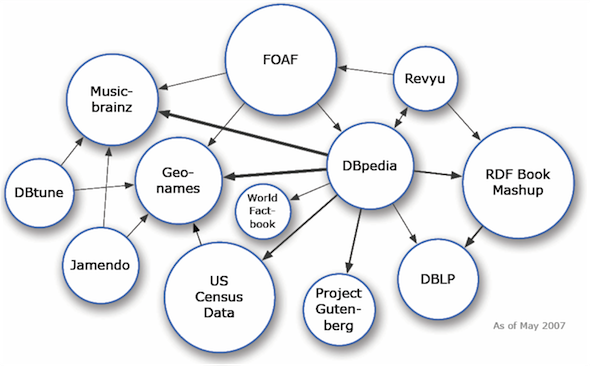
\includegraphics[width=0.9\textwidth]{img/lod-cloud2007.png}
\caption{LOD cloud as of May, 2007}
\label{fig:lodcloud2007}
\end{figure}

Linked data is a new research field that uses RDF model to manipulate data on the Web, interconnect it with other data and consume it in a variety of applications showcasing it's benefits. The resulting ``Web of data'' has started being populated with geospatial data, as proved by the efforts in [cite-efforts]. Those efforts and initiatives follow the vision of the \textit{Semantic Geospatial Web} promotes by Max Egenhofer in \cite{egenhofer12} challenging GIS researchers to contribute to the Semantic Web effort by creating geospatial ontologies, query languages and processing techniques adapted to geospatial information on the Web. In \cite{koubarakis12}, the authors mentioned many research topics in the area of linked geospatial data, that some are listed herein:

\begin{enumerate}


\item \textit{Vocabularies:} How do we model geospatial information on the Web? How do we assess geospatial ontologies? How to serialize complex geometry? 
\item \textit{Query languages:} How do we write efficient queries that target geospatial Web? How do store and index geodata in RDF ?
\item \textit{Datasets:} How do we extract and convert geodata to expose on the Web? What are the best practices for representing complex geometries on the Web? How can we integrate fully compatibility of CRSs on datasets? 
\item \textit{Publication:} How can we develop scalable frameworks for covering the workflow of publishing geodata? What are the appropriate triple stores for handling geodata? What are the metrics to use for interconnecting different geodata resources on the Web?  
\item \textit{Applications and user interfaces:} How do we generate interesting visualizations of linked geospatial data? What are appropriate high-level APIs that ease the development of user interfaces for geospatial data? Can we rely on existing map platforms such as Google Maps, Bing Maps or OpenSteetMap?
\end{enumerate}

In this thesis we mainly focus on the first, third and fifth of the above topics, and acknowledge existing efforts on the rest of the topic. 

\begin{figure}[ht!]
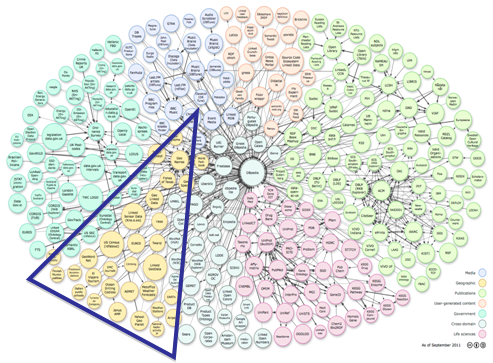
\includegraphics[scale=0.9]{img/lod-diagram-2011.png}
\caption{LOD cloud as of August, 2011}
\label{fig:lodcloud2011}
\end{figure}

\begin{figure}[ht!]
\centering{
\includegraphics[scale=0.1]{img/LODcloud2014.pdf}
\caption{LOD cloud as of April, 2014}
\label{fig:lodcloud2014}
}
\end{figure}



\section{Research Questions}
\label{sec:questions}

The Web is currently in a transition phase. After having been accessible on personal computers, it is now 
quickly moving to more and more ubiquity and entering in every part and moment of our lives. New 
devices and new ways to use them are being created. The ubiquity of the Web also creates an unseen 
abundance of information. Data is flowing onto the Web, created by users, generated by sensors, and 
stored in ever growing data farms. Geographic data is widely present on the web as they are used for location 
of Point of Interest. At the same time, many organizations are moving from legacy data stored in their databases
to structured data on the web. Structured data is already present in the many databases, metadata attached to medias, and in the millions of spreadsheets created everyday across the world. 

The ubiquity of the Web is creating an unseen abundance of information. Data is flowing onto the Web, created by users, generated by sensors, and stored in ever growing data farms. Geographic data is widely present on the web as they are used for location of Point of Interest. At the same time, many organizations are moving from legacy data stored in their databases to structured data on the web. Structured data is already present in the many databases, metadata attached to medias, and in the millions of spreadsheets created everyday across the world.

Our concern was to tackle the problematic in two directions : 
\begin{itemize}
\item (i) Geographic Information on the Web of data: as an application of the life-cycle of publishing geodata.
\item (ii) Visualization tools for building innovative applications consuming structured data: as for leveraging the process of creating applications on-top of semantic data to highlight some relevant knowledge to the users.

\end{itemize}



\section{Contributions}
\label{sec:contributions}

\subsection{Contributions on Geodata}
Regarding this aspect of our research, we have achieved the following tasks:
 \begin{itemize}
  \item We have proposed an ontology describing features and point of interest for the French territory, by reusing existing taxonomy (GeOnto) and aligning it to other related vocabularies of the domain.
 \item We have made a comparative study of the triple stores, comparing their capability to store spatial information and their implementation of topological functions with respect to the ones 
existing in OGC\footnote{http://www.opengeospatial.org/} standards.
 \item We presented the output of those ideas in two conferences: the French Knowledge Engineering Community \cite{atemezing2012a} and the Terra Cognita workshop at the Semantic Web Conference \cite{atemezing2012b}.

\end{itemize}

\subsection{Modeling Geographic Information in LOD} \label{model}
The need for geolocation is crucial for many applications for both human and software agents. More and more data is opened and interlinked using Linked Data principles, and it is worth modeling geographic data efficiently by reusing as much as possible from existing ontologies or vocabularies that describe both the geospatial features and their shapes. In the first part of our work, we survey different modeling approaches used by the Geographic Information System (GIS) and the Linked Open Data (LOD) communities. Our aim is to contribute to the actual efforts in representing geographic objects with attributes such as location, points of interest (POI), and addresses on the web of data. We focus on the French territory and we provide examples of representative vocabularies that can be used for describing geographic objects. We propose some alignments between various vocabularies (DBpedia, GeoNames, Schema.org, LinkedGeoData, Foursquare, etc.) in order to enable interoperability while interconnecting French geodata with other datasets. In France, there is  currently a joint effort to publish geographic information in RDF (Resource Description Framework) and interlink them with relevant datasets. GeOnto is an ontology describing geospatial features for the French territory. We have proposed to align GeOnto with other popular vocabularies in the geospatial domain, using Silk for schema mapping and we have evaluated the results. We studied how to extend the model to take into account efficient modeling for complex geometries. By doing so, tackle the complex geometry representation issues in the Web of Data, describing the state of implementations of geo-spatial functions in triple stores and comparing them to the new GeoSPARQL standard.  We finally made some recommendations and advocate for the reuse of the NeoGeo ontology within GeOnto to better address the IGN requirements.

\subsection{Visualization Tools in Linked Government Data} \label{visu}

We first review the numerous applications that have been developed on top of datasets that have been opened by governments (UK, USA, France) and local authorities. We have then derived and proposed some use cases (8 UCs) that can be developed to consume data from the different main providers in the French level: INSEE, DILA, IGN, FING, etc. We mention that the most interesting UCs are the ones which show the added value of having interconnected datasets. These UCs,  developed and deployed, can be useful to show the benefits of Linked Data in a variety of domains such as Education, Tourism, Cultural Heritage, Civil administrations, Judicial Court, Medicine, etc. 

Regarding tools used for visualization, we have divided them in two categories, providing for each of them relevant examples: (i)-tools that operate over RDF data, (ii) and tools that operate over other structured format. We then provide some basic criteria for assessing a given visualization tool, with some weight attached to each of the criterion. 

We have contributed  on : 
\begin{itemize}
\item (i)- Designing and implementing vocabularies for describing complex geometries with different coordinate systems, with direct application to the French administrative unit
\item (ii)- Proposing a method to harmonize prefixes on the web of data  with two services: LOV\footnote{http://lov.okfn.org/dataset/lov/} and prefix.cc\footnote{http://prefix.cc}. 
\end{itemize}

\subsection{Contributions on visualizations}
Concerning our contributions on visualizations, we have contributed by:
\begin{itemize}
\item Building an application of the French first round elections using data from the data.gouv.fr and other public institutions.
\item Building an application for conference events (confomaton) with their associated media reconciled from many social platform (instagram, twitter, etc.)
\item Building a vocabulary for structuring applications on the Web of data
\item Implementing a first version of a visualization module aiming at recommending a suitable tool for easing the creation of an application according to the dataset.

\end{itemize}

\subsection{Contributions to Standards}
We contribute to the W3C Government Linked Data Working Group (GLD WG)\footnote{http://www.w3.org/2011/gld/} activity since July, 2011.  The objective of the Working Group is to \textit{``provide standards and other information which help governments around the world publish their data as effective and usable Linked Data using Semantic Web technologies''}. %The GLD WG has its regular call of 60 min every Thursday, with some extra calls for specific works. We were present in the second Face-to-Face (2F2F) meeting on 25-26 Jan 2012, at DERI Galway. 

The group has three main task forces:
\begin{itemize}
\item \textbf{Task Force 1} aims to create a linked data community directory\footnote{http://dir.w3.org} and to maintain it on-line about deployments, vendors, contractors, end-user applications. In this work, we contribute to define the requirements and providing data for the French organizations in the directory.
\item \textbf{Task Force 2} aims at providing \textbf{``Best Practices''} for Publishing Linked Data by producing recommendations regarding vocabulary selection, URI construction, Linked Data Cookbook, versioning, stability and provenance. Here, we are actively preparing a check list to help government to select and re-use vocabularies in their project. We have also proposed our vision of the Linked Open Data Life cycle, best practices to construction URI and how to publish data which has multiple versions over a time period. We are also involved in defining relevant terms in the Linked Data Glossary\footnote{https://dvcs.w3.org/hg/gld/raw-file/default/glossary/index.html} working Note. Apart from contributing in many sections of the document ``Best Practices for Publishing Linked Data'', we edited the working note \cite{wood2012}.

\item \textbf{Task Force 3} goal is to  provide relevant vocabularies to be used by governments or local authorities in their process of exposing their data. The scope of the vocabularies are: the description of people, business, data catalogue, organization, legal entity and statistical data. 
\end{itemize}


\section{Thesis Outline}
\label{sec:thesis-structure}